\chapter{Determination of Tensile Force of Bolts}
\section{Nomenclature}
\begin{tabular}[t]{lp{8cm}}
		$ [F_{cb}] $ & tension force at failure of common bolt, $ N $\\
		$ [F_{sb}] $ & tension force at failure of steel bolt, $ N $\\
		$ [\sigma_{cb}] $ & tension at failure of common bolt, $ MPa $\\
		$ [\sigma_{sb}] $ & tension at failure of steel bolt, $ MPa $\\
		$ d $ & nominal diameter of M8 bolt, $ mm $\\
		$ F_c $ & tension force of hydraulic cylinder\\
		$ F_{cb} $ & tension force at failure of common bolt, $ N $\\
		$ F_{sb} $ & tension force at failure of steel bolt, $ N $\\
\end{tabular}

\section{Aim}
\begin{enumerate}
	\item Help students understand more clearly about tensile force of some types of steels, the relation between central $ M_k $ and localized strain of material.
	\item Help students approach methods, measuring devices in determining tensile force.
\end{enumerate}

\section{Safety Procedures}
\begin{enumerate}
	\item Safeguard is compulsory when straining the bolt.
	\item Close the machine gate when operating.
\end{enumerate}

\section{Experimental Report}
\begin{table}[ht]
	\centering
	\renewcommand{\arraystretch}{1.5}
	\rowcolors{3}{}{lightgray!20}
	
	\begin{tabular}{cR{2.75cm}R{2.75cm}}\toprule
		\multirow{2}{*}{No.} & \multicolumn{2}{c}{Experiment with $d=8\unit{mm}$} \\ \cmidrule{2-3}
		& $F_{sb}$         & $F_{cb}$               \\ \midrule
		1                    & 33898            & 37377                           \\
		2                    & 33574            & 37053                           \\
		3                    & 34211            & 36426                           \\
		4                    & 33727            & 37053                           \\
		5                    & 34211            & 36426                           \\
		Avg              & 33323.4          & 36867                           \\ \bottomrule
	\end{tabular}
	\caption{Tension force at failure of common and steel bolts}
\end{table}

\section{Data plot}
\begin{figure}[ht]
	\centering
	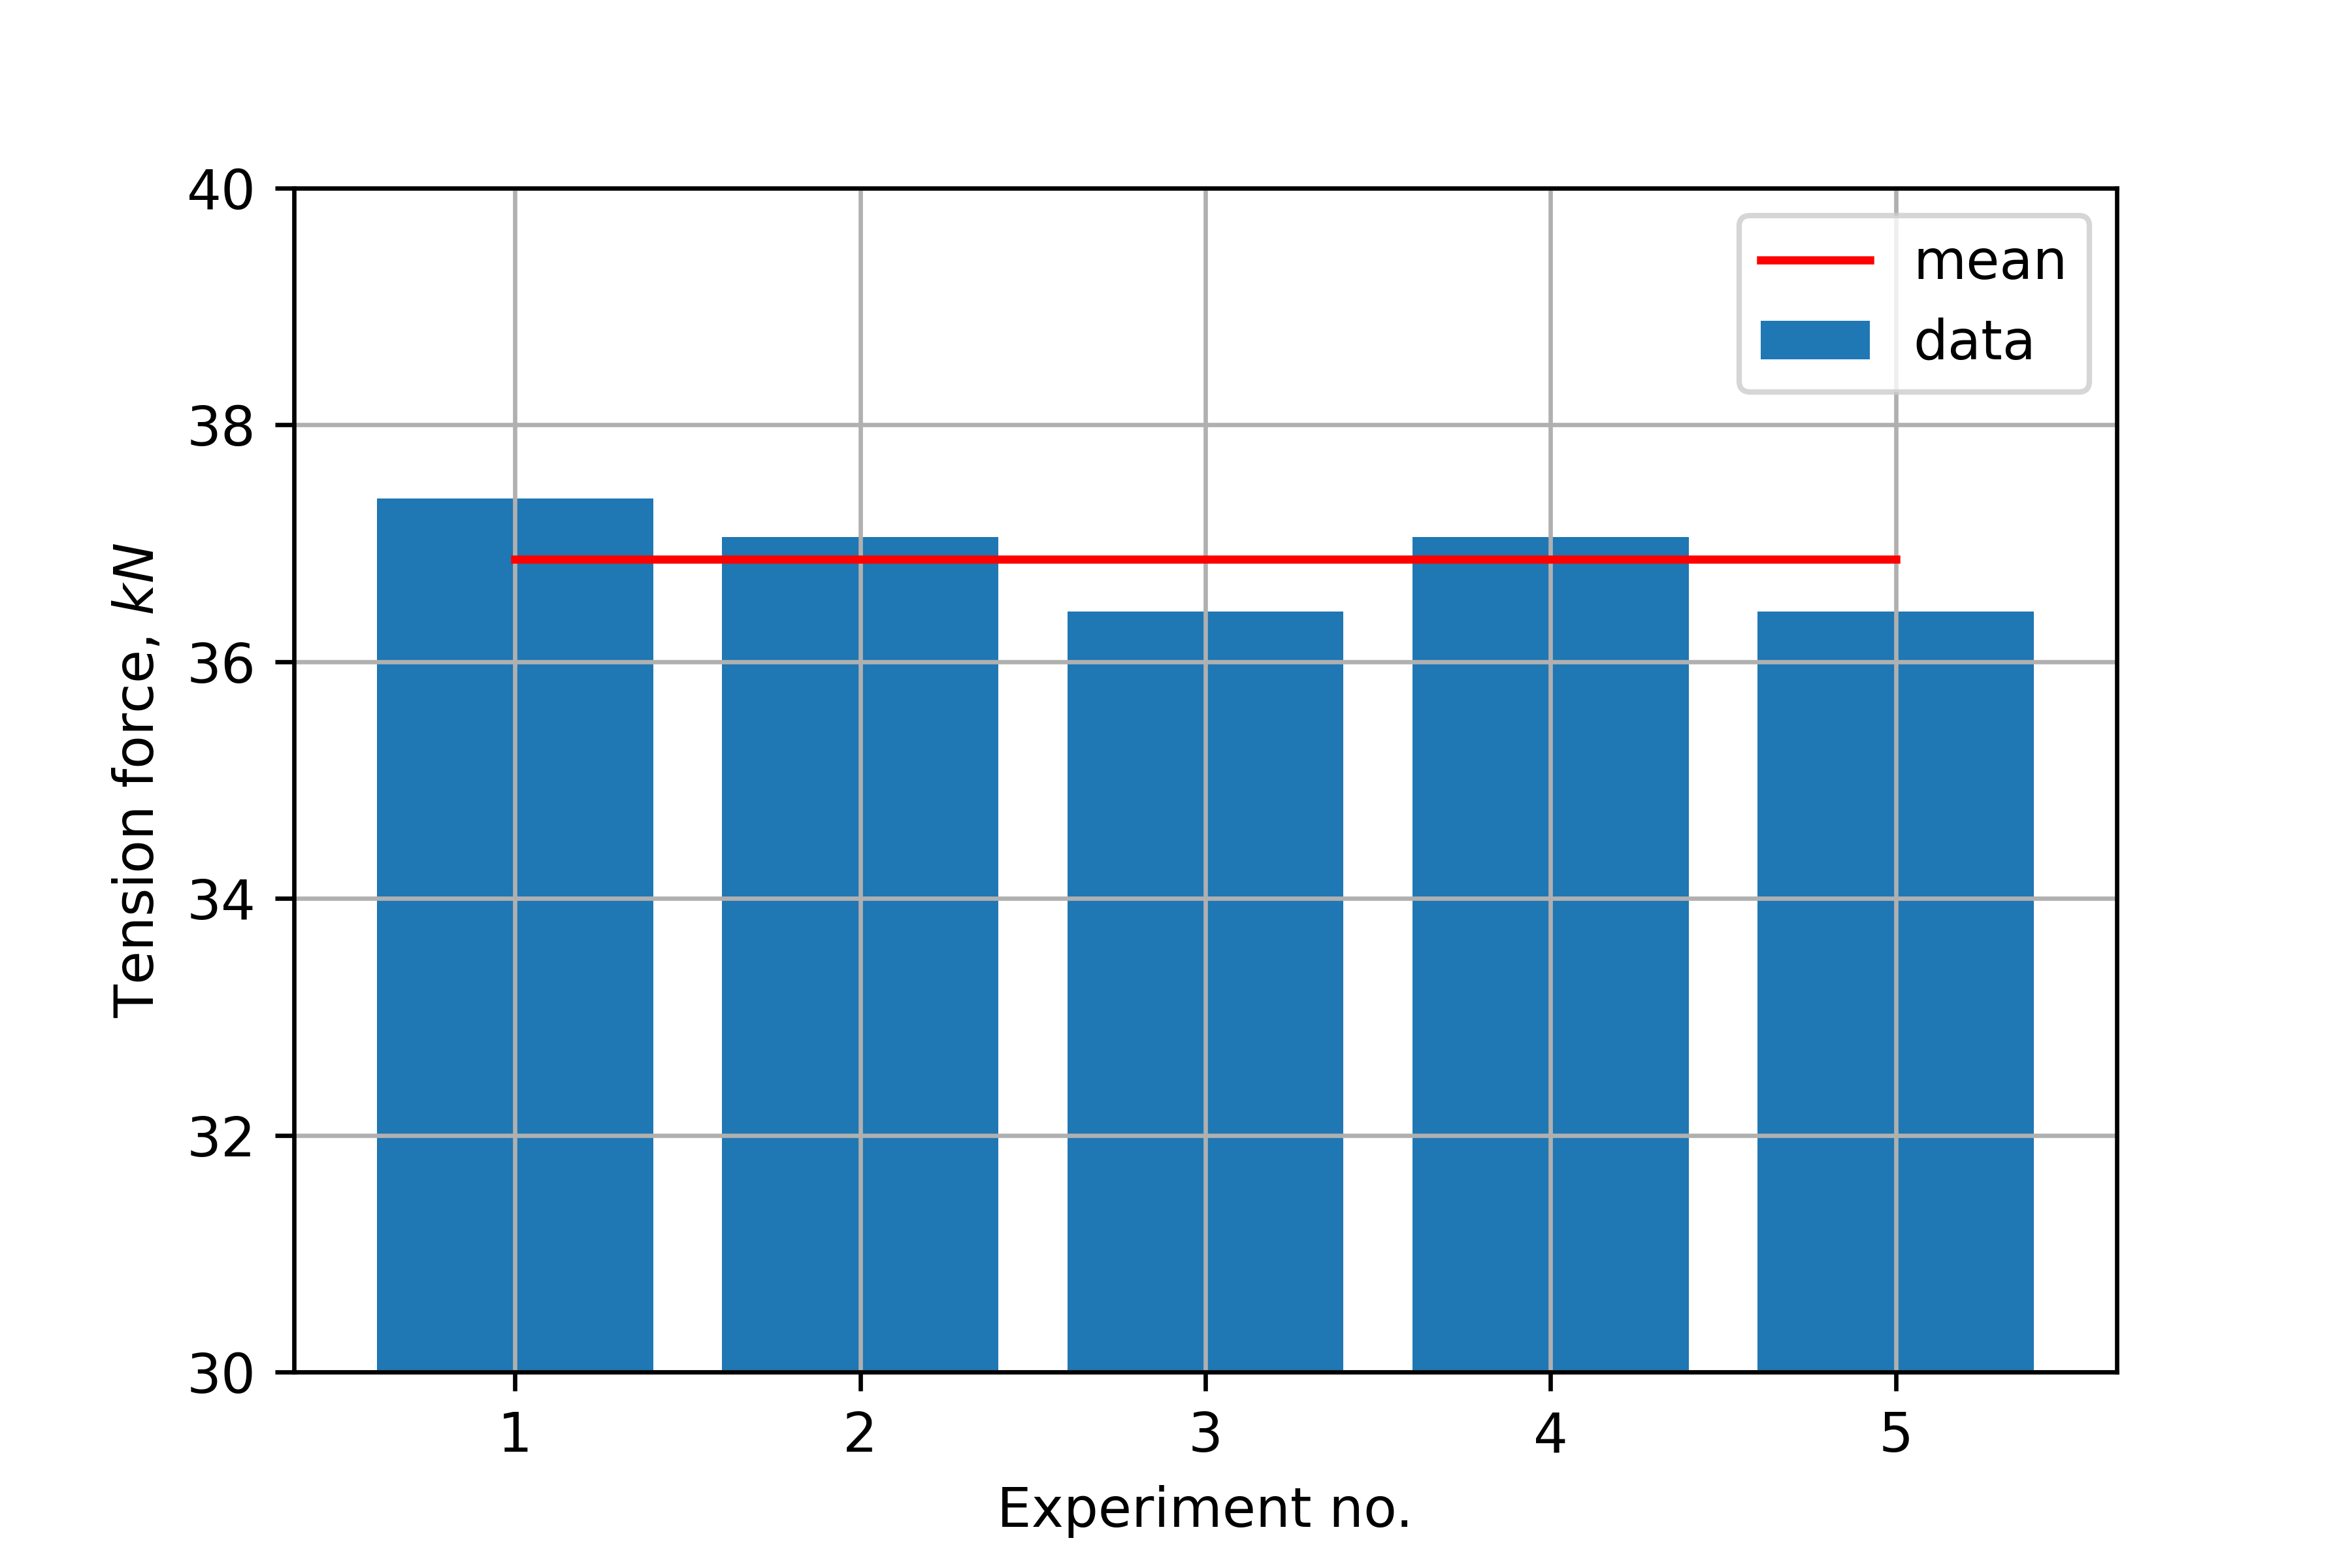
\includegraphics[width=140mm]{Exp2cb.png}
	\caption{Tension force at failure of common bolt}
\end{figure}
\begin{figure}[ht]
	\centering
	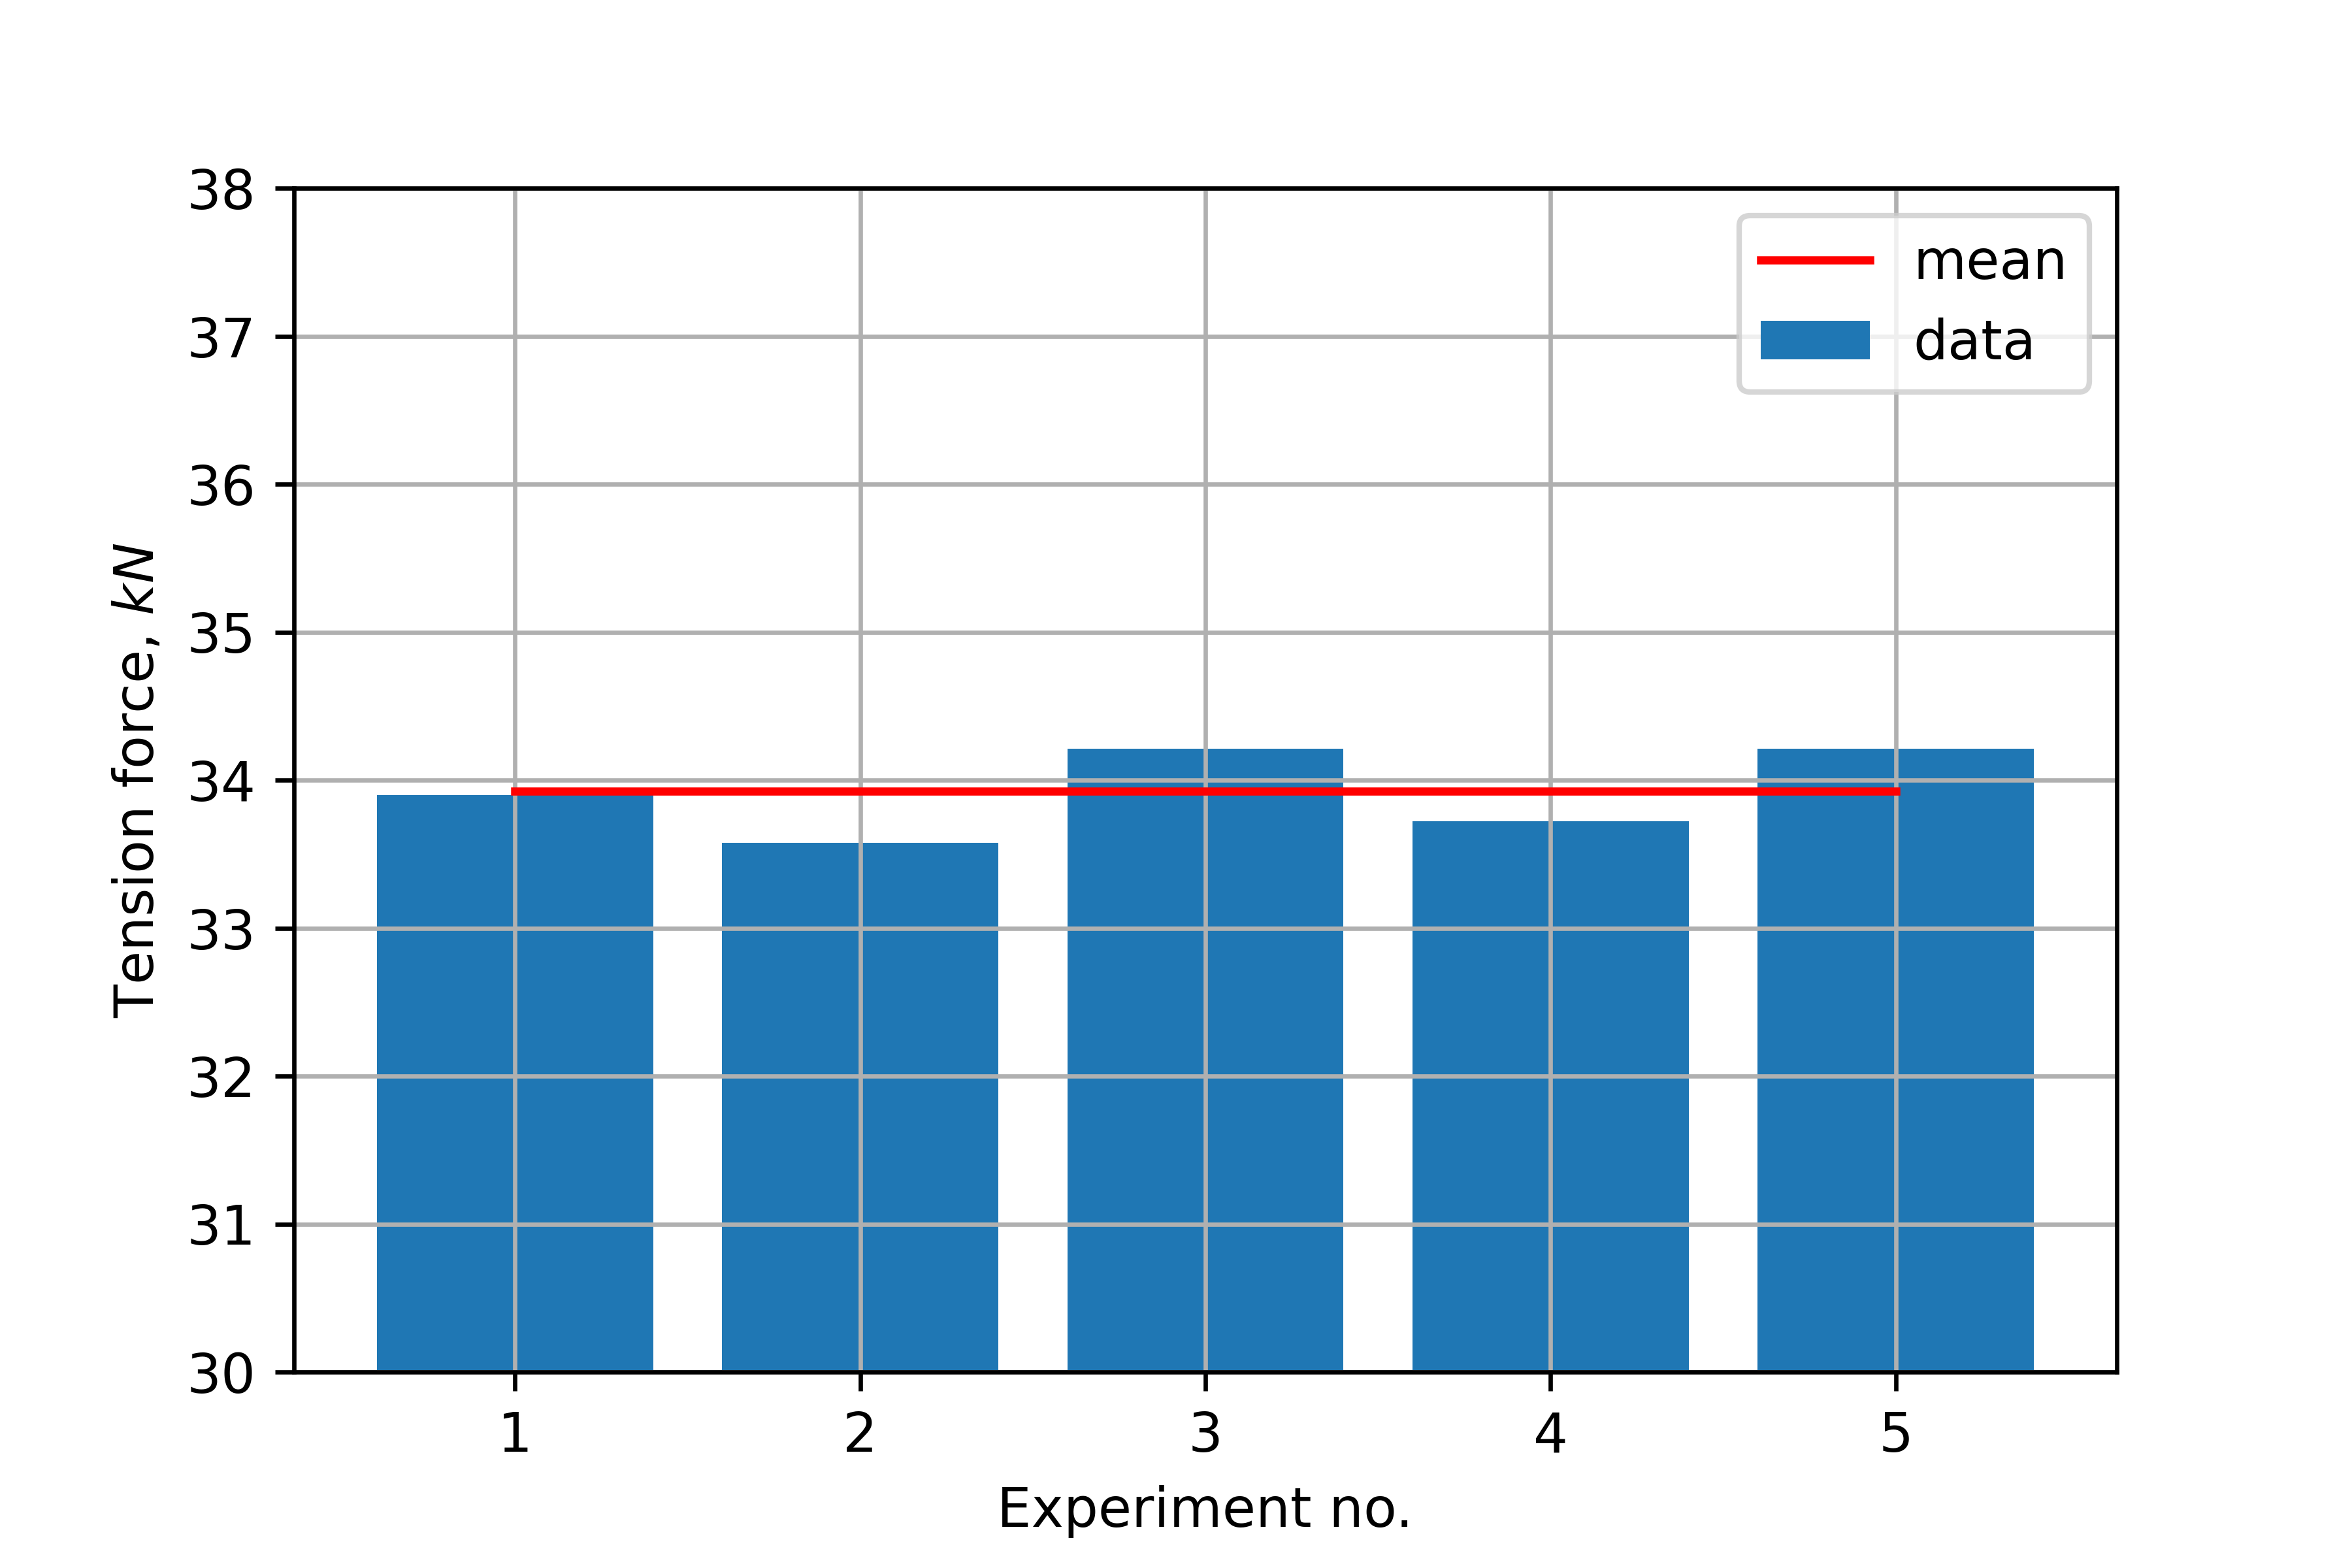
\includegraphics[width=140mm]{Exp2sb.png}
	\caption{Tension force at failure of steel bolt}
\end{figure}
%\newpage
%\section{Discussion and conclusions}
%
%\section{Review questions}